\documentclass[
blockverticalspace=-0.75cm
]{tikzposter}
\geometry{paperwidth=24in, paperheight=36in}

% 2 feet wide by 3 feet tall
% 24in=2ft, 36in=3ft

% 3 feet wide by 4 feet tall
% 36in=3ft, 48in=4ft

\makeatletter
\setlength{\TP@visibletextwidth}{22in}
\setlength{\TP@visibletextheight}{34in}
\makeatother

\usepackage[utf8]{inputenc}
\usepackage{tikz}
\usepackage{xcolor}

\usepackage{setspace}
\onehalfspacing

\usepackage[pangram]{blindtext}
\usepackage{comment}
\usetikzlibrary{arrows.meta}
\usepackage{minted}

\newcommand{\largearrow}{-{Latex[length=3mm,width=5mm]}}

% Colors sourced from https://www.redcross.org/content/dam/redcross/atg/PDFs/BrandPoster.pdf
\definecolor{coolgray}{HTML}{6D6E70}
\definecolor{redcrossred}{HTML}{ED1B2E}


\tikzset{%
  >={Latex[width=2mm,length=2mm]},
  % Specifications for style of nodes:
            base/.style = {rectangle, rounded corners, draw=black,
                           minimum width=8cm, minimum height=0.5cm,
                           text centered, font=\sffamily},
		startstyle/.style = {base, fill=blue!30},
		astyle/.style = {base, fill=red!30},
		bstyle/.style = {base, fill=green!30},
		cstyle/.style = {base, minimum width=2.5cm, fill=orange!15,
                           font=\ttfamily},
}

\usecolorstyle[colorOne=coolgray,colorTwo=white,colorThree=redcrossred]{Germany}
\tikzposterlatexaffectionproofoff

\title{\fontsize{44pt}{18pt}
    Twitter Fire Scraper}
\author{Research Team}
\date{\today}
\institute{Illinois Institute of Technology}

\begin{document}

\maketitle

\begin{columns}

\column{1}
\vspace{-2cm}
\block{Overview}
{
    {
    \fontsize{46pt}{20pt}\selectfont
    Twitter's content spans the entire spectrum of human thought and first hand information. Our team built a model to classify tweets into categories relevant to humanitarian incidents that the American Red Cross could respond to. In our project, we explore different classification models that could be used to identify true positives from the Twitter scraper's keyword searches in order to reduce the time and memory required by the American Red Cross to refine its keyword and account searches for the scraper.       
    }
}


\end{columns}

\vspace{-1cm}

\begin{columns}

    \column{0.5}
    \block{Model Performance}
    {\vspace{-1cm}
        \begin{tikzfigure}
        \begin{center}
            
            Accuracy of the 4 models tested:
            
         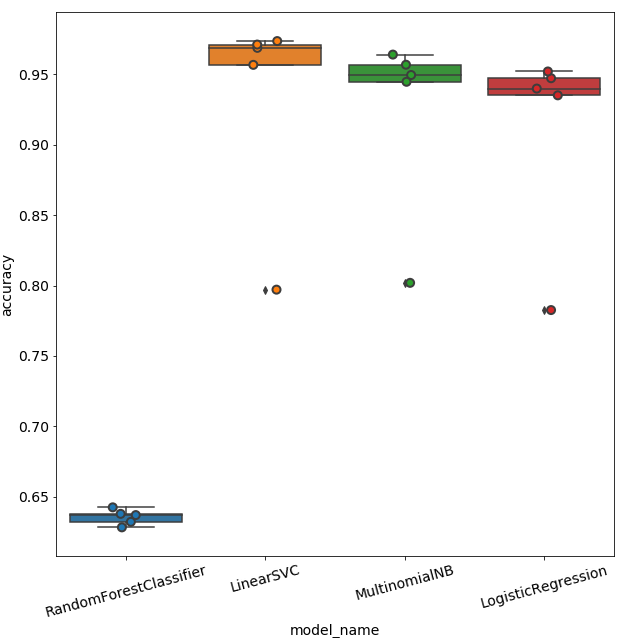
\includegraphics[width=0.3\textwidth]{Poster_Pics/results_large_text.png}
        \end{center}   
        \end{tikzfigure}
        \vspace{-1cm}
        \begin{tikzfigure}
            
        
        \vspace{1cm}    
        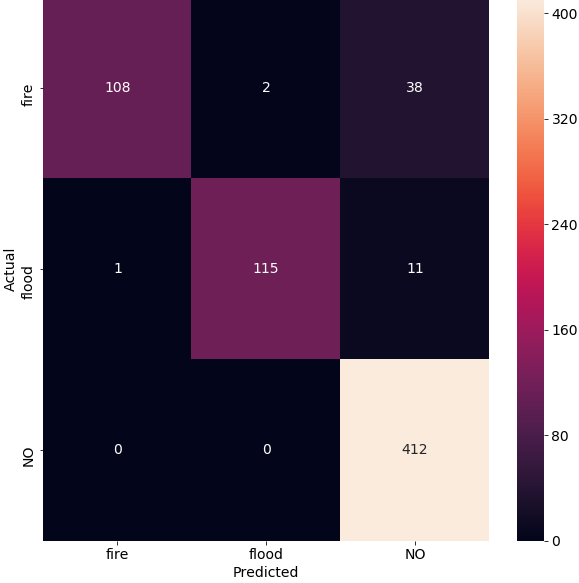
\includegraphics[width=0.3\textwidth]{Poster_Pics/confusion.png}
        \begin{center}
            \begin{caption}
                LinearSVC Confusion Matrixs
            \end{caption}
        \end{center}
        \end{tikzfigure}
    {
    \fontsize{40pt}{14pt}\selectfont
     The confusion matrix shows not only the accuracy of the model, but also where the models misclassified the most, and what categories the models misclassified to. Based on unseen tweets, the model reads the text and outputs a prediction for that text ``fire'', ``flood'', or ``NO''. Then it compares it to its actual label.\\
    }
    }
    \column{0.5}
    \block{Recall and Precision Results}
    {
        \begin{tikzfigure}%[Caption]
            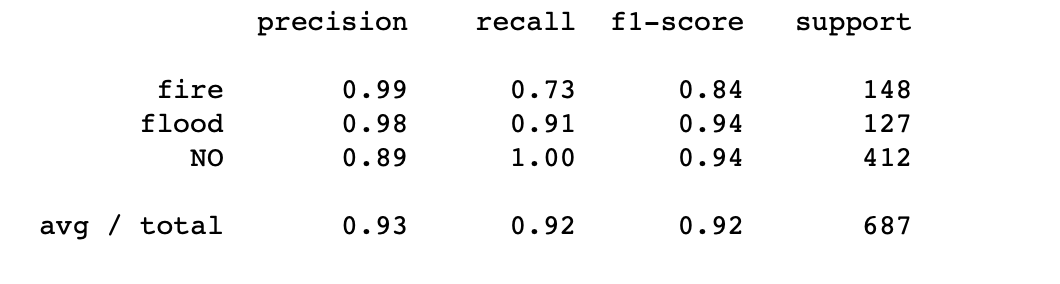
\includegraphics[width=0.3\textwidth]{Poster_Pics/stats.png}
        \end{tikzfigure}
        {
        \fontsize{40pt}{14pt}\selectfont
        We chose to analyze the precision and recall scores of the model as these essentially are measures of the true positive rate of the model. Precision is defined to be:
        
        \vspace{0.5cm}
        \begin{equation}
            Precision = \frac{Total\ True\ Positives}{Total\ Positives}
        \end{equation}
        \vspace{0.5cm}

        Recall is defined to be:
        
        \vspace{0.5 cm}
        \begin{equation}
            Recall = \frac{Total\ True\ Positives}{Total\ Correctly\ Classified}
        \end{equation}
        
        \vspace{0.5 cm}
        The F1-score is defined to be:
        \begin{equation}
            F_1 = 2 * \frac{precision * recall}{precision+recall}
        \end{equation}
        \vspace{0.5 cm}
        
        simply the harmonic mean of precision and recall. It could be seen as a weighted accuracy score, as it weights the accuracy if the categories are not balanced. Overall the model performs decently given the current scores and the f1-score. To maximize recall, we will work on implementing an active learning strategy to train the model on tweets the American Red Cross sees on a daily basis.
        }
    }
    
  %  \block{Future Work}
   % {
    %\fontsize{40pt}{14pt}\selectfont
%    \begin{enumerate}
%        \item Integrate the classification tool into the Twitter Scraper.
%        \item Implement an active learning algorithm into the Twitter Scraper and text classification tool. This will help maximize the $F_1$ score and help train the model to identify tweets that specifically relate to incidents in the Chicago-area.
%        \item Build a system into the MongoDB database that calculates a reliability index for accounts that are frequently queried by the Scraper and classification tool.
%        \item Work with Twitter to increase the frequency and amount of tweets we are able to collect.
%        \item Expand our collection of tweets for data analysis.
%    \end{enumerate}
%    }
    
    
    \block{}% Logos
    {
        \vspace{-2.25cm}
        \begin{tikzfigure}
        
\includegraphics[scale=0.50]{Poster_Pics/Logos.png}
        \end{tikzfigure} 
    }

    
\end{columns}

\end{document}
